\documentclass{article}
\usepackage{v-test-paper}
\usepackage{pgfplots}
\renewcommand{\frac}[2]{\dfrac{#1}{#2}}
\begin{document}
\begin{center}
    \textsc{Introductory Exercise 6.1}
\end{center}
\begin{enumerate}
    \item “A lift is descending with increasing speed”. What are the directions of velocity and acceleration in the given statement?
    \item Velocity and acceleration of a particle at some instant are
    \[ v = (3\hat{i} - 4\hat{j} + 2\hat{k}) m/s \quad \text{and} \quad a = (2\hat{i} + \hat{j} - 2\hat{k}) m/s^2 \]
    \begin{enumerate}
        \item What is the value of dot product of $\vec{v}$ and $\vec{a}$ at the given instant?
        \item What is the angle between $\vec{v}$ and $\vec{a}$, acute, obtuse or 90\textdegree?
        \item At the given instant, whether speed of the particle is increasing, decreasing or constant?
    \end{enumerate}
\end{enumerate}

\vspace*{10 mm}
\begin{center}
    \textsc{Introductory Exercise 6.2}
\end{center}
\begin{enumerate}
    \item Velocity and acceleration of a particle are
    \[ v = (2\hat{i} - 4\hat{j}) \, \text{m/s} \quad \text{and} \quad a = (-2\hat{i} + 4\hat{j}) \, \text{m/s}^2 \]
    Which type of motion is this?
    \item Velocity and acceleration of a particle are
    \[ v = (2\hat{i}) \, \text{m/s} \quad \text{and} \quad a = (4\hat{i} + t^2\hat{j}) \, \text{m/s}^2 \]
    where \( t \) is the time. Which type of motion is this?
    \item In the above question, can we use \( v = u + at \) equation directly?
\end{enumerate}

\vspace*{10 mm}
\begin{center}
    \textsc{Introductory Exercise 6.3}
\end{center}
\begin{enumerate}
    \item Average speed is always equal to magnitude of average velocity. Is this statement true or false?
    \item When a particle moves with constant velocity its average velocity, its instantaneous velocity and its speed all are equal. Is this statement true or false?
    \item A stone is released from an elevator going up with an acceleration of \( g/2 \). What is the acceleration of the stone just after release?
    \item A clock has its second hand 2.0 cm long. Find the average speed and modulus of average velocity of the tip of the second hand in 15 s.
    \item 
    \begin{enumerate}
        \item Is it possible to be accelerating if you are travelling at constant speed?
        \item Is it possible to move on a curved path with zero acceleration, constant acceleration, variable acceleration?
    \end{enumerate}
    \item A particle is moving in a circle of radius 4 cm with constant speed of 1 cm/s. Find
    \begin{enumerate}
        \item time period of the particle.
        \item average speed, average velocity and average acceleration in a time interval from \( t = 0 \) to \( t = T/4 \). Here, \( T \) is the time period of the particle. Give only their magnitudes.
    \end{enumerate}
\end{enumerate}

\vspace*{10 mm}
\begin{center}
    \textsc{Introductory Exercise 6.4}
\end{center}
\begin{enumerate}
    \item A particle moves in a straight line with constant speed of \(4 \text{ m/s} \) for \(2 \text{ s}\), then with \(6 \text{ m/s}\) for \(3 \text{ s}\). Find the average speed of the particle in the given time interval.
    \item A particle travels half of the time with constant speed \(2 \text{ m/s}\). In remaining half of the time it travels, \(\frac{1}{4}\)th distance with constant speed of \(4 \text{ m/s}\) and \(\frac{3}{4}\)th distance with \(6 \text{ m/s}\). Find average speed during the complete journey.
\end{enumerate}

\pagebreak
\begin{center}
    \textsc{Introductory Exercise 6.5}
\end{center}
\begin{enumerate}
    \item Prove the relation, \( s_t = u + at - \frac{1}{2} a \).
    \item Equation \( s_t = u + at - \frac{1}{2} a \) does not seem dimensionally correct, why?
    \item A particle is projected vertically upwards. What is the value of acceleration
    \begin{enumerate}
        \item[(i)] during upward journey,
        \item[(ii)] during downward journey and
        \item[(iii)] at highest point?
    \end{enumerate}
    \item A ball is thrown vertically upwards. Which quantity remains constant among, speed, kinetic energy, velocity and acceleration?
    \item A particle is projected vertically upwards with an initial velocity of 40 m/s. Find the displacement and distance covered by the particle in 6 s. Take \( g = 10 m/s^2 \).
    \item A particle moves rectilinearly with initial velocity \( u \) and constant acceleration \( a \). Find the average velocity of the particle in a time interval from \( t = 0 \) to \( t = t \) second of its motion.
    \item A particle moves in a straight line with uniform acceleration. Its velocity at time \( t = 0 \) is \( v_1 \), and at time \( t = t \) is \( v_2 \). The average velocity of the particle in this time interval is \( \frac{v_1 + v_2}{2} \).
    \begin{enumerate}
        \item Is this statement true or false?
    \end{enumerate}
    \item Find the average velocity of a particle released from rest from a height of 125 m over a time interval till it strikes the ground. Take \( g = 10 m/s^2 \).
    \item A particle starts with an initial velocity 2.5 m/s along the positive x-direction and it accelerates uniformly at the rate 0.50 m/s\(^2\).
    \begin{enumerate}
        \item[(a)] Find the distance travelled by it in the first two seconds
        \item[(b)] How much time does it take to reach the velocity 7.5 m/s?
        \item[(c)] How much distance will it cover in reaching the velocity 7.5 m/s?
    \end{enumerate}
    \item A ball is projected vertically upward with a speed of 50 m/s. Find 
    \begin{enumerate}
        \item[(a)] the maximum height,
        \item[(b)] the time to reach the maximum height,
        \item[(c)] the speed at half the maximum height. Take \( g = 10 m/s^2 \).
    \end{enumerate}
\end{enumerate}


\vspace*{10 mm}
\begin{center}
    \textsc{Introductory Exercise 6.6}
\end{center}
\begin{enumerate}
    \item Velocity (in m/s) of a particle moving along x-axis varies with time as, $v = (10 + 5t - t^2)$
    \begin{enumerate}
        \item acceleration of particle at $t = 2$ s and
        \item x-coordinate of particle at $t = 3$ s
    \end{enumerate}

    \item A particle is moving with a velocity of $v = (3 + 6t + 9t^2)$ cm/s. Find out
    \begin{enumerate}
        \item the acceleration of the particle at $t = 3$ s.
        \item the displacement of the particle in the interval $t = 5$ s to $t = 8$ s.
    \end{enumerate}

    \item The motion of a particle along a straight line is described by the function $x = (2t - 3)^2$, where x is in metres and t is in seconds. Find
    \begin{enumerate}
        \item the position, velocity and acceleration at $t = 2$ s.
        \item the velocity of the particle at origin.
    \end{enumerate}

    \item x-coordinate of a particle moving along this axis is $x = (2 + t^2 + 2t^3)$. Here, x is in metres and t in seconds. Find
    \begin{enumerate}
        \item position of particle from where it started its journey,
        \item initial velocity of particle and (c) acceleration of particle at $t = 2$ s.
    \end{enumerate}

    \item The velocity of a particle moving in a straight line is directly proportional to $3/4$th power of time elapsed. How does its displacement and acceleration depend on time?
\end{enumerate}

\pagebreak
\begin{center}
    \textsc{Introductory Exercise 6.7}
\end{center}
\begin{enumerate}
    \item Velocity of a particle at time \( t = 0 \) is 2 m/s. A constant acceleration of 2 m/s\(^2\) acts on the particle for 2 s at an angle of \( 60^\circ \) with its initial velocity. Find the magnitude of velocity and displacement of particle at the end of \( t = 2 \)s.
    \item Velocity of a particle at any time \( t \) is \( \mathbf{v} = (2i + 2tj) \) m/s. Find acceleration and displacement of particle at \( t = 1 \)s. Can we apply \( \mathbf{v} = \mathbf{u} + \mathbf{a}t \) or not?
    \item Acceleration of a particle in x-y plane varies with time as 
    \[
    \mathbf{a} = (2ti + 3t^2j) \text{ m/s}^2
    \]
    At time \( t = 0 \), velocity of particle is 2 m/s along positive x-direction and particle starts from origin. Find velocity and coordinates of particle at \( t = 1 \)s.
\end{enumerate}

\vspace*{10 mm}
\begin{center}
    \textsc{Introductory Exercise 6.8}
\end{center}
\begin{enumerate}
    \item Two particles A and B are moving along x-axis. Their x-coordinate versus time graphs are as shown below
    \begin{center}
        \begin{tikzpicture}
            \draw[->] (0,0) -- (6,0) node[anchor=north] {$t$ (s)};
            \draw[->] (0,0) -- (0,4) node[anchor=east] {$x$ (m)};
            \draw[thick] (0,1) -- (4,3) node[anchor=south west] {A};
            \draw[thick] (0,0.5) -- (4,3.5) node[anchor=south west] {B};
            \draw[dashed] (0,3) node[anchor=east] {30} -- (4,3);
            \draw[dashed] (4,0) node[anchor=north] {8} -- (4,3);
            \draw[dashed] (0,1) node[anchor=east] {10} -- (2,1);
            \draw[dashed] (2,0) node[anchor=north] {4} -- (2,1);
            \draw[dashed] (0,0.5) -- (2,0.5);
        \end{tikzpicture}
        Fig. 6.35
    \end{center}

    \begin{enumerate}
        \item Find the time when the particles start their journey and the x-coordinate at that time.
        \item Find velocities of the two particles.
        \item When and where the particles strike with each other.
    \end{enumerate}

    \item The velocity of a car as a function of time is shown in Fig. 6.36. Find the distance travelled by the car in 8 s and its acceleration.

    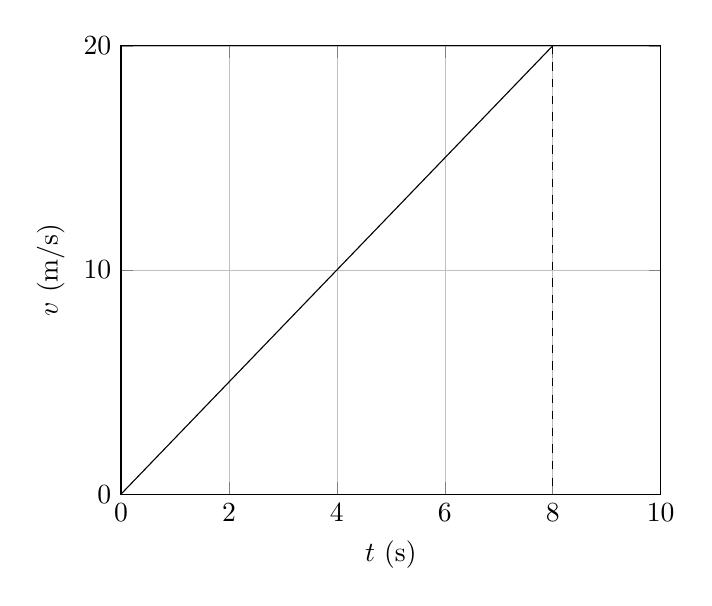
\begin{tikzpicture}
        \begin{axis}[
            xlabel={$t$ (s)},
            ylabel={$v$ (m/s)},
            xmin=0, xmax=10,
            ymin=0, ymax=20,
            xtick={0,2,...,10},
            ytick={0,10,20},
            grid=both,
            grid style={line width=.1pt, draw=gray!10},
            major grid style={line width=.2pt,draw=gray!50},
        ]
        % Velocity-time graph
        \addplot[domain=0:8, samples=2] {2.5*x};
        \draw[dashed] (axis cs:8,20) -- (axis cs:8,0);
        \end{axis}
    \end{tikzpicture}

    \item Fig. 6.37 shows the graph of velocity versus time for a particle going along the x-axis. Find (a) acceleration, (b) the distance travelled in 0 to 10 s and (c) the displacement in 0 to 10 s.

    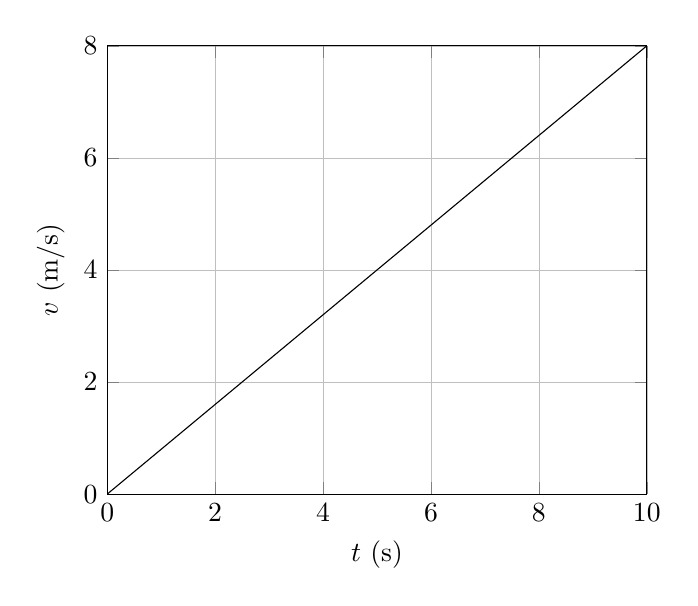
\begin{tikzpicture}
        \begin{axis}[
            xlabel={$t$ (s)},
            ylabel={$v$ (m/s)},
            xmin=0, xmax=10,
            ymin=0, ymax=8,
            xtick={0,2,...,10},
            ytick={0,2,...,8},
            grid=both,
            grid style={line width=.1pt, draw=gray!10},
            major grid style={line width=.2pt,draw=gray!50},
        ]
        % Velocity-time graph
        \addplot[domain=0:10, samples=2] {0.8*x};
        \end{axis}
    \end{tikzpicture}

    \item Fig. 6.38 shows the graph of the x-coordinate of a particle going along the x-axis as a function of time. Find (a) the average velocity during 0 to 10 s, (b) instantaneous velocity at 2, 5, 8 and 12 s.

    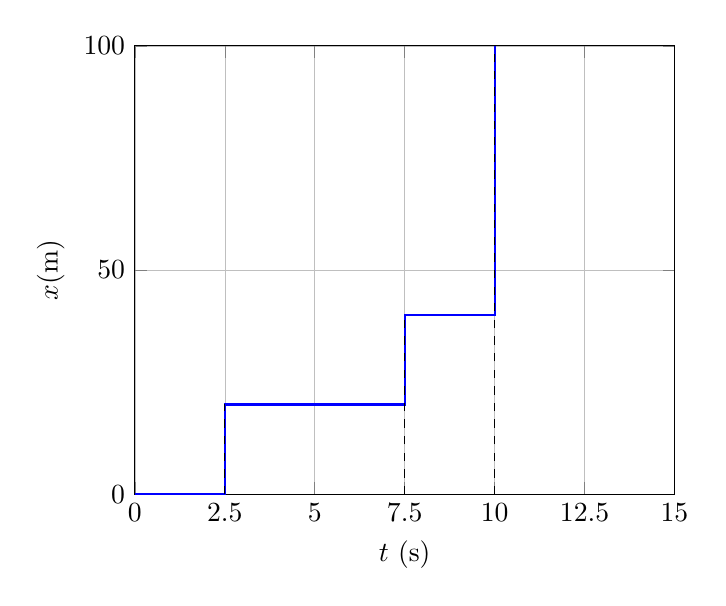
\begin{tikzpicture}
        \begin{axis}[
            xlabel={$t$ (s)},
            ylabel={$x$(m)},
            xmin=0, xmax=15,
            ymin=0, ymax=100,
            xtick={0,2.5,...,15},
            ytick={0,50,100},
            grid=both,
            grid style={line width=.1pt, draw=gray!10},
            major grid style={line width=.2pt,draw=gray!50},
        ]
        % x-t graph with piecewise constant velocity
        \addplot+[const plot, no marks, thick] coordinates {(0,0) (2.5,20) (7.5,40) (10,100)};
        \draw[dashed] (axis cs:2.5,0) -- (axis cs:2.5,20);
        \draw[dashed] (axis cs:7.5,0) -- (axis cs:7.5,40);
        \draw[dashed] (axis cs:10,0) -- (axis cs:10,100);
        \end{axis}
    \end{tikzpicture}

    \item From the velocity-time plot shown in Fig. 6.39, find the distance travelled by the particle during the first 40 s. Also find the average velocity during this period.

    \begin{tikzpicture}
        \begin{axis}[
            xlabel={$t$ (s)},
            ylabel={$v$ (m/s)},
            xmin=0, xmax=40,
            ymin=-5, ymax=5,
            xtick={0,10,...,40},
            ytick={-5,0,5},
            grid=both,
            grid style={line width=.1pt, draw=gray!10},
            major grid style={line width=.2pt,draw=gray!50},
        ]
        % Velocity-time graph with positive and negative velocity segments
        \addplot+[const plot, no marks] coordinates {(0,0) (20,5) (40,-5)};
        \draw[dashed] (axis cs:20,0) -- (axis cs:20,5);
        \end{axis}
    \end{tikzpicture}
\end{enumerate}


\vspace*{10 mm}
\begin{center}
    \textsc{Introductory Exercise 6.9}
\end{center}
\begin{enumerate}
    \item Two particles are moving along x-axis. Their x-coordinate versus time graph are as shown below.
    
    \begin{tikzpicture}
    \draw[->] (0,0) -- (6,0) node[right] {$t$ (s)};
    \draw[->] (0,0) -- (0,3) node[above] {$x$ (m)};
    \draw[dashed] (0,2.5) node[left] {12} -- (2.5,2.5) node[above right] {B} -- (2.5,0) node[below] {5};
    \draw (2.5,2.5) -- (5,2) node[above right] {A};
    \end{tikzpicture}
    
    Find velocity of A w.r.t. B.
  
    \item Two balls A and B are projected vertically upwards with different velocities. What is the relative acceleration between them?
  
    \item A river 400 m wide is flowing at a rate of 2.0 m/s. A boat is sailing at a velocity of 10.0 m/s with respect to the water in a direction perpendicular to the river. 
    \begin{enumerate}
      \item Find the time taken by the boat to reach the opposite bank.
      \item How far from the point directly opposite to the starting point does the boat reach the opposite bank?
    \end{enumerate}
  
    \item An aeroplane has to go from a point A to another point B, 500 km away due 30° east of north. Wind is blowing due north at a speed of 20 m/s. The steering-speed of the plane is 150 m/s.
    \begin{enumerate}
      \item Find the direction in which the pilot should head the plane to reach the point B.
      \item Find the time taken by the plane to go from A to B.
    \end{enumerate}
  
    \item A man crosses a river in a boat. If he cross the river in minimum time he takes 10 min with a drift 120 m. If he crosses the river taking shortest path, he takes 12.5 min, find
    \begin{enumerate}
      \item width of the river
      \item velocity of the boat with respect to water
      \item speed of the current
    \end{enumerate}
  
    \item A river is 20 m wide. River speed is 3 m/s. A boat starts with velocity $2\sqrt{2}$ m/s at angle $45^\circ$ from the river current (relative to river)
    \begin{enumerate}
      \item Find the time taken by the boat to reach the opposite bank.
      \item How far from the point directly opposite to the starting point does the boat reach the opposite bank?
    \end{enumerate}
  \end{enumerate}



  \begin{enumerate}
    \item \textbf{Assertion}: Velocity and acceleration of a particle are given as, $\vec{v} = i - j$ and $\vec{a} = -2i + 2j$.
    
    This is a two dimensional motion with constant acceleration.
    
    \textbf{Reason}: Velocity and acceleration are two constant vectors.
    
    \item \textbf{Assertion}: Displacement-time graph is a parabola corresponding to straight line velocity-time graph.
    
    \textbf{Reason}: Velocity and acceleration graph is a parabola corresponding to straight line velocity-time graph.
    
    \item \textbf{Assertion}: If $v = u + at$ then $s = ut + \frac{1}{2}at^2$
    
    \textbf{Reason}: In $v-t$ graph shown in figure, average velocity in time interval from 0 to $t_0$ depends only on $v_0$. It is independent of $t_0$.
    
    % Diagram for question 3 using TikZ
    \begin{tikzpicture}
    % Define axes
    \draw[->] (0,0) -- (3,0) node[right] {$t$};
    \draw[->] (0,0) -- (0,3) node[above] {$v$};

    % Define graph
    \draw (0,0.5) node[left] {$v_0$} -- (2,0.5) -- (2,0) node[below] {$t_0$};

    % Define points
    \fill (0,0.5) circle (1pt);
    \fill (2,0.5) circle (1pt);
    \end{tikzpicture}
    
    \item \textbf{Assertion}: We know the relation $a = \frac{dv}{dt}$. Therefore, if velocity of a particle is zero, then acceleration is also zero.
    
    \textbf{Reason}: In the above equation, $a$ is the instantaneous acceleration.
    
    \item \textbf{Assertion}: Speed of a particle may decrease, even if acceleration is increasing.
    
    \textbf{Reason}: This will happen if acceleration is positive.
    
    \item \textbf{Assertion}: Starting from rest with zero acceleration if acceleration of particle increases at a constant rate of $2 \text{ m/s}^3$ then velocity should increase at constant rate of $1 \text{ m/s}^2$.
    
    \textbf{Reason}: For the given condition.
    \[
    \frac{da}{dt} = 2 \text{ m/s}^3
    \]
    Therefore,
    \[
    a = 2t
    \]
    
    \item \textbf{Assertion}: Average velocity can't be zero in case of uniform acceleration.
    
    \textbf{Reason}: For average velocity to be zero, a non zero velocity should not remain constant.
\end{enumerate}

\begin{tikzpicture}
    \draw[->] (0,0) -- (4,0) node[anchor=north] {$t$};
    \draw[->] (0,0) -- (0,3) node[anchor=east] {$s$};
    \draw (0,2) to[out=0,in=135] (2,1.5) node[anchor=south] {$A$} to[out=-45,in=180] (4,0.5) node[anchor=west] {$B$};
    \draw[dotted] (2,1.5) -- (2,0) node[anchor=north] {$t_A$};
    \draw[dotted] (2,1.5) -- (0,1.5) node[anchor=east] {$s_A$};
    \fill (2,1.5) circle (1.5pt);
\end{tikzpicture}



\begin{center}
    \textsc{Single Correct Answer Type}
\end{center}

\begin{enumerate}
    \item A stone is released from a rising balloon accelerating upward with acceleration \( a \). The acceleration of the stone just after the release is
    \begin{tasks}(4)
        \task \( a \) upward
        \task \( g \) downward
        \task \( (g + a) \) downward
        \task \( (g - a) \) downward
    \end{tasks}

    \item A ball is thrown vertically upwards from the ground. If \( T_1 \) and \( T_2 \) are the respective time taken in going up and coming down, and the air resistance is not ignored, then
    \begin{tasks}(4)
        \task \( T_1 > T_2 \)
        \task \( T_1 = T_2 \)
        \task \( T_1 < T_2 \)
        \task nothing can be said
    \end{tasks}

    \item The length of a seconds hand in watch is 1 cm. The change in velocity of its tip in 15 s is
    \begin{tasks}(4)
        \task zero
        \task \( \frac{\pi}{30} \) cm/s
        \task \( \frac{\pi}{30\sqrt{2}} \) cm/s
        \task \( \frac{\pi}{15} \) cm/s
    \end{tasks}

    \item When a ball is thrown up vertically with velocity \( v_0 \), it reaches a maximum height of \( h \). If one wishes to triple the maximum height then the ball should be thrown with velocity
    \begin{tasks}(4)
        \task \( \sqrt{3} v_0 \)
        \task \( 3 v_0 \)
        \task \( 9 v_0 \)
        \task \( \frac{3}{2} v_0 \)
    \end{tasks}


    \item During the first 18 min of a 60 min trip, a car has an average speed of 11 m s\(^{-1}\). What should be the average speed for remaining 42 min so that car is having an average speed of 21 m s\(^{-1}\) for the entire trip?
    \begin{tasks}(4)
        \task 25.3 m s\(^{-1}\)
        \task 29.2 m s\(^{-1}\)
        \task 31 m s\(^{-1}\)
        \task 35.6 m s\(^{-1}\)
    \end{tasks}
    \item A particle moves along a straight line. Its position at any instant is given by \( x = 32t - \frac{8}{3}t^3 \) where \( x \) is in metres and \( t \) in seconds. Find the acceleration of the particle at the instant when particle is at rest.
    \begin{tasks}(4)
        \task -16 m s\(^{-2}\)
        \task -32 m s\(^{-2}\)
        \task 32 m s\(^{-2}\)
        \task 16 m s\(^{-2}\)
    \end{tasks}
    \item The acceleration of a particle is increasing linearly with time \( t \) as \( bt \). The particle starts from the origin with an initial velocity \( v_0 \). The distance travelled by the particle in time \( t \) will be
    \begin{tasks}(4)
        \task \( v_0 t + \frac{1}{6}bt^2 \)
        \task \( v_0 t + \frac{1}{2}bt^3 \)
        \task \( v_0 t + \frac{1}{3}bt^2 \)
        \task \( v_0 t + \frac{1}{2}bt^2 \)
    \end{tasks}
    \item Water drops fall at regular intervals from a tap 5 m above the ground. The third drop is leaving the tap, the instant the first drop touches the ground. How far above the ground is the second drop at that instant. ( \( g = 10 \) m s\(^{-2}\) )
    \begin{tasks}(4)
        \task 1.25 m
        \task 2.50 m
        \task 3.75 m
        \task 4.00 m
    \end{tasks}
    \item A stone is dropped from the top of a tower and one second later, a second stone is thrown vertically downward with a velocity 20 m s\(^{-1}\). The second stone will overtake the first after travelling a distance of \( g = 10 \) m s\(^{-2}\)
    \begin{tasks}(4)
        \task 11.25 m
        \task 15 m
        \task 19.5 m
        \task none of these
    \end{tasks}
    \item A particle moves in the \( xy \)-plane with velocity \( \vec{u} \). If \( u_x = 8t - 2 \) and \( u_y = 2 \). If it passes through the point \( x = 14 \) and \( y = 4 \) at \( t = 2 \) s, the equation of the path is
    \begin{tasks}(4)
        \task \( y = x^2 - y - 2 \)
        \task \( x = y^2 + y - 6 \)
        \task \( x = y^2 - y - 6 \)
        \task None of these
    \end{tasks}
    % Diagram using TikZ for question 10 - A simple representation is provided, but for complex diagrams, further details would be required
    % Please adjust or extend the TikZ code as needed to match the complete details of the diagram in the textbook.
    \begin{tikzpicture}
    \draw[->] (0,0) -- (5,0) node[anchor=north] {\(x\)};
    \draw[->] (0,0) -- (0,5) node[anchor=east] {\(y\)};
    \draw[thick] (0,0) parabola bend (2,4) (4,0);
    \filldraw (2,4) circle (2pt) node[anchor=south] {\((14,4)\)};
    \draw[dotted] (2,0) node[anchor=north] {14} -- (2,4) -- (0,4) node[anchor=east] {4};
    \end{tikzpicture}
    \item The horizontal and vertical displacements of a particle moving along a curved line are given by \( x = 5t \) and \( y = 2t^2 + t \). The displacement which its velocity vector makes an angle of \( 45^\circ \) with the horizontal is
    \begin{tasks}(4)
        \task 0.5 s
        \task 1 s
        \task 2 s
        \task 1.5 s
    \end{tasks}
    \item A ball is released from the top of a tower of height \( h \) metre. It takes \( T \) second to reach the ground. What is the position of the ball in \( T/3 \) second?
    \begin{tasks}(4)
        \task \( \frac{h}{9} \) metre from the ground
        \task \( \frac{(7h/9)}{9} \) metre from the ground
        \task \( \frac{(8h/9)}{9} \) metre from the ground
        \task \( \frac{(17h/18)}{9} \) metre from the ground
    \end{tasks}
    \item An ant is at a corner of a cubical room of side \( a \). The ant can move with a constant speed \( u \). The minimum time taken to reach the farthest corner of the cube is
    \begin{tasks}(4)
        \task \( \frac{3a}{u} \)
        \task \( \frac{\sqrt{3}a}{u} \)
        \task \( \frac{\sqrt{5}a}{u} \)
        \task \( \frac{(\sqrt{2} + 1)a}{u} \)
    \end{tasks}

    \item A lift starts from rest. Its acceleration is plotted against time. When it comes to rest its height above its starting point is 
    \begin{tasks}(4)
        \task \(20 \text{ m}\)
        \task \(64 \text{ m}\)
        \task \(32 \text{ m}\)
        \task \(36 \text{ m}\)
    \end{tasks}
  
    \item A lift performs the first part of its ascent with uniform acceleration \(a\) and the remaining with uniform retardation \(2a\). If \(t\) is the time of ascent, find the depth of the shaft.
    \begin{tasks}(4)
        \task \(\frac{at^2}{4}\)
        \task \(\frac{2at^2}{3}\)
        \task \(\frac{at^2}{2}\)
        \task \(\frac{at^2}{8}\)
    \end{tasks}
  
    \item Two objects are moving along the same straight line. They cross a point A with an acceleration \(a\), 2a and velocity \(2u\), \(u\) at time \(t = 0\). The distance moved by the object when one overtakes the other is
    \begin{tasks}(4)
        \task \(\frac{6u^2}{a}\)
        \task \(\frac{2u^2}{a}\)
        \task \(\frac{4u^2}{a}\)
        \task \(\frac{8u^2}{a}\)
    \end{tasks}
  
    \item A car is moving horizontally along a straight line with constant speed 30 m/s\(^{-1}\). A particle is to be fired vertically upwards from the moving cart in such a way that it returns to the same point from where it was projected after the cart has moved 80 m. At what speed (relative to the cart) must the projectile be fired? (Take \(g = 10 \text{ ms}^{-2}\))
    \begin{tasks}(2)
        \task \(10 \text{ ms}^{-1}\)
        \task \(10\sqrt{8} \text{ ms}^{-1}\)
        \task \(\frac{40}{3} \text{ ms}^{-1}\)
        \task None of these
    \end{tasks}
  
    \item The figure shows velocity--time graph of a particle moving along a straight line. Identify the correct statement.
    \begin{tasks}
        \task The particle starts from the origin
        \task The particle crosses it initial position at \(t = 2s\)
        \task The average speed of the particle in the time interval, \(0 \leq t \leq 2s\) is zero
        \task All of the above
    \end{tasks}

% TikZ diagram for Question 18
\begin{tikzpicture}
    \draw [->] (0,0) -- (4,0) node [right] {$t(s)$};
    \draw [->] (0,-3) -- (0,2) node [above] {$v(m/s)$};
    \draw (0,0) -- (1,1.5) -- (2,0) -- (3,-2.5);
    \draw[dotted] (1,0) -- (1,1.5);
    \draw[dotted] (2,0) -- (2,-2.5);
    \draw[dotted] (3,0) -- (3,-2.5);
    \foreach \x in {0,1,2,3}
       \draw (\x cm,1pt) -- (\x cm,-1pt) node[anchor=north] {$\x$};
    \foreach \y/\ytext in {-2/-20, -1/-10, 1/10}
       \draw (1pt,\y cm) -- (-1pt,\y cm) node[anchor=east] {$\ytext$};
\end{tikzpicture}
  
    \item A ball is thrown vertically upwards from the ground and a student gazing out of the window sees it moving upward past him at 10 m/s\(^{-1}\). The window is at 15 m above the ground level. The velocity of ball 3 s after it was projected from the ground is (Take \(g = 10 \text{ ms}^{-2}\))
    \begin{tasks}(2)
        \task \(10 \text{ ms}^{-1}\), up
        \task \(20 \text{ ms}^{-1}\), up
        \task \(20 \text{ ms}^{-1}\), down
        \task \(10 \text{ ms}^{-1}\), down
    \end{tasks}
    
    \item A body starts moving with a velocity \(v_0 = 10 \text{ ms}^{-1}\). It experiences a retardation equal to \(0.2v^2\). Its velocity after 2s is given by
    \begin{tasks}(4)
        \task \(+ 2 \text{ ms}^{-1}\)
        \task \(+ 4 \text{ ms}^{-1}\)
        \task \(- 2 \text{ ms}^{-1}\)
        \task \(+ 6 \text{ ms}^{-1}\)
    \end{tasks}

    \item Two trains are moving with velocities \(u_1 = 10\ \text{ms}^{-1}\) and \(u_2 = 20\ \text{ms}^{-1}\) on the same track in opposite directions. After the application of brakes if their retarding rates are \(a_1 = 2\ \text{ms}^{-2}\) and \(a_2 = 1\ \text{ms}^{-2}\) respectively, then the minimum distance of separation between the trains to avoid collision is 
    \begin{tasks}(4)
        \task \(150\ \text{m}\)
        \task \(225\ \text{m}\)
        \task \(450\ \text{m}\)
        \task \(300\ \text{m}\)
    \end{tasks}

    \item Two identical balls are shot upward one after another at an interval of 2s along the same vertical line with same initial velocity of \(40\ \text{ms}^{-1}\). The height at which the balls collide is
    \begin{tasks}(4)
        \task \(50\ \text{m}\)
        \task \(75\ \text{m}\)
        \task \(100\ \text{m}\)
        \task \(125\ \text{m}\)
    \end{tasks}

    \item A particle is projected vertically upwards and reaches the maximum height \(H\) in time \(T\). The height of the particle at any time \(t (T)\) will be
    \begin{tasks}(2)
        \task \(g t (T - t^2)\)
        \task \(H - g (t - T)^2\)
        \task \(\frac{1}{2} g (t - T)^2\)
        \task \(H - \frac{1}{2} g (T - t)^2\)
    \end{tasks}

    \item A particle moves along the curve \(y = \frac{x^2}{2}\). Here \(x\) varies with time \(t\) as \(x = \frac{t^2}{2}\). Where \(x\) and \(y\) are measured in metres and \(t\) in seconds. At \(t = 2\) s, the velocity of the particle (\(\text{ms}^{-1}\)) is
    \begin{tasks}(4)
        \task \(4i + 6j\)
        \task \(4i + 4j\)
        \task \(2i + 4j\)
        \task \(2i + 2j\)
    \end{tasks}

    \item If the displacement of a particle varies with time as \(x = \sqrt{t} + 3\)
    \begin{tasks}
        \task velocity of the particle is inversely proportional to \(t\)
        \task velocity of the particle varies linearly with \(t\)
        \task velocity of particle is proportional to \(\sqrt{t}\)
        \task initial velocity of the particle is zero
    \end{tasks}

    \item The graph describes an airplane's acceleration during its take-off run. The airplane's velocity when it lifts off at \(t = 20\) s is
    % TikZ diagram for question 26
    \begin{tikzpicture}
        \begin{axis}[
            axis lines=left,
            xlabel={\(t\ (s)\)},
            ylabel={\(a\ (\text{ms}^{-2})\)},
            ymin=0, ymax=6,
            xmin=0, xmax=30,
            xtick={0,10,20},
            ytick={0,3,5},
            ymajorgrids=true,
            grid style=dashed,
        ]
            \addplot[
                jump mark left,
                thick,
                mark=*, 
                mark options={solid}
                ] coordinates {(0,0) (10,5) (20,5) (20,0)};
            \draw[dashed] (axis cs:20,0) -- (axis cs:20,5) node[pos=0.5,right] {};
        \end{axis}
    \end{tikzpicture}

    \begin{tasks}(4)
        \task \(40\ \text{ms}^{-1}\)
        \task \(50\ \text{ms}^{-1}\)
        \task \(90\ \text{ms}^{-1}\)
        \task \(180\ \text{ms}^{-1}\)
    \end{tasks}

    \item A particle moving in a straight line has velocity-displacement equation as \(v = 5\sqrt{1 + s}\). Here \(v\) is in \(\text{ms}^{-1}\) and \(s\) in metres. Select the correct alternative.
    \begin{tasks}
        \task Particle is initially at rest
        \task Initially velocity of the particle is \(5\ \text{ms}^{-1}\) and the particle has a constant acceleration of \(12.5\ \text{ms}^{-2}\)
        \task Particle moves with a uniform velocity
        \task None of the above
    \end{tasks}

    \item A particle is thrown upwards from ground. It experiences a constant resistance force which can produce a retardation of \(2 \, \text{ms}^{-2}\). The ratio of time of ascent to time of descent is (g = 10 ms\(^{-2}\)) 
    \begin{tasks}(2) % Adjust the number in parenthesis to set the number of columns of answers
        \task \(1 : 1\)
        \task \( \frac{2}{\sqrt{3}} \)
        \task \(\frac{2}{3}\)
        \task \( \frac{\sqrt{3}}{2} \)
    \end{tasks}
    
    \item A body of mass 10 kg is being acted upon by a force \(3t^2\) and an opposing constant force of 32 N. The initial speed is \(10 \, \text{ms}^{-1}\). The velocity of body after 5 s is
    \begin{tasks}(2)
        \task \(14.5 \, \text{ms}^{-1}\)
        \task \(6.5 \, \text{ms}^{-1}\)
        \task \(3.5 \, \text{ms}^{-1}\)
        \task \(4.5 \, \text{ms}^{-1}\)
    \end{tasks}
    
    \item A stone is thrown vertically upwards. When stone is at a height half of its maximum height, its speed is \(10 \, \text{ms}^{-1}\); then the maximum height attained by the stone is (g = \(10 \, \text{ms}^{-2}\))
    \begin{tasks}(2)
        \task \(25 \, \text{m}\)
        \task \(10 \, \text{m}\)
        \task \(15 \, \text{m}\)
        \task \(20 \, \text{m}\)
    \end{tasks}
    
\end{enumerate}

\begin{center}
    \textsc{Subjective Questions}
\end{center}


\begin{enumerate}
    \item 
    \begin{enumerate}
        \item What does $\frac{dv}{dt}$ and $\frac{d|v|}{dt}$ represent?
        \item Can these be equal?
    \end{enumerate}
    \item The coordinates of a particle moving in x-y plane at any time t are $(2t, t^2)$. Find
    \begin{enumerate}
        \item the trajectory of the particle,
        \item velocity of particle at time t and
        \item acceleration of particle at any time t.
    \end{enumerate}
    \item A farmer has to go 500 m due north, 400 m due east and 200 m due south to reach his field. If he takes 20 min to reach the field.
    \begin{enumerate}
        \item What distance he has to walk to reach the field?
        \item What is the displacement from his house to the field?
        \item What is the average speed of farmer during the walk?
        \item What is the average velocity of farmer during the walk?
    \end{enumerate}
    \item A rocket is fired vertically up from the ground with a resultant vertical acceleration of $10 ms^{-2}$.
    \begin{enumerate}
        \item What is the maximum height reached?
        \item After how much time from then will the maximum height be reached? (Take g = $10 ms^{-2}$)
    \end{enumerate}
    \item A particle is projected upwards from the roof of a tower 60 m high with velocity 20 m/s. Find
    \begin{enumerate}
        \item the average speed and
        \item average velocity of the particle up to an instant when it strikes the ground. (Take g = $10 ms^{-2}$)
    \end{enumerate}
    \item A block moves in a straight line with velocity u for time $t_0$. Then, its velocity becomes 2u for next $t_0$ time. Finally, its velocity becomes 3u for time T. If average velocity during the complete journey was 2.5 u, then find T in terms of $t_0$.
    \item A particle starting from rest has a constant acceleration of $4 ms^{-2}$ for 4 s. It then retards uniformly for next 8 s and comes to rest. Find during the motion of particle 
    \begin{enumerate}
        \item average acceleration
        \item average speed and 
        \item average velocity.
    \end{enumerate}
    \item A particle moves in a circle of radius $R = \frac{22}{21} m$ with constant speed 1m/s. Find,
    \begin{enumerate}
        \item magnitude of average velocity and 
        \item magnitude of average acceleration in 2 s.
    \end{enumerate}
    \item Two particles A and B start moving simultaneously along the line joining them in the same direction with acceleration of 1 $ms^{-2}$ and 2 $ms^{-2}$ and speeds 3 m/s and 1 m/s respectively. Initially, A is 10 m behind B. What is the minimum distance between them?
    \item Two diamonds begin a free fall from rest from the same height, 1.0 s apart. How long after the first diamond begins to fall will the two diamonds be 10 m apart? Take g = $10 ms^{-2}$.
    \item Two bodies are projected vertically upwards from one point with the same initial velocity $v_0$. The second body is projected $t_s$ after the first. How long after will the bodies meet?
    \item Displacement-time graph of a particle moving in a straight line is as shown in figure.
    \begin{center}
        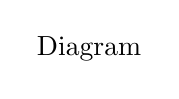
\begin{tikzpicture}
            \node {Diagram};
        \end{tikzpicture}
    \end{center}
    
    \begin{enumerate}
        \item Find the sign of velocity in regions oa, ab, bc and cd.
        \item Find the sign of acceleration in the above region.
    \end{enumerate}
    \item Velocity-time graph of a particle moving in a straight line is shown in figure. In the time interval from t = 0 to t = 14 s, find
    \begin{enumerate}
        \item average velocity and
        \item average speed of the particle.
    \end{enumerate}
    \item A person walks up a stalled 15 m long escalator in 90 s. When standing on the same escalator, now moving, the person is carried up in 60 s. How much time would it take that person to walk up the moving escalator? Does the answer depend on the length of the escalator?
    \item Figure shows the displacement-time graph of a particle moving in a straight line. Find the signs of velocity and acceleration of particle at time t = $t_1$ and t = $t_2$.
    \begin{center}
        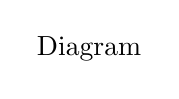
\begin{tikzpicture}
            \node {Diagram};
        \end{tikzpicture}
    \end{center}
    \item Velocity of a particle moving along positive x-direction is $v = (40 - 10t)$ m/s. Here, t is in seconds. At time t = 0, the x-coordinate of particle is zero. Find the time when the particle is at a distance of 60 m from origin.



% Question 17
\item Velocity-time graph of a particle moving in a straight line is shown in figure. Plot the corresponding displacement-time graph of the particle if at time \( t = 0 \), displacement \( s = 0 \).

% TikZ environment for diagram in Question 17
\begin{center}
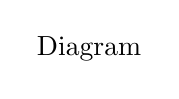
\begin{tikzpicture}
\node {Diagram};
\end{tikzpicture}
\end{center}

% Question 18
\item Acceleration-time graph of a particle moving in a straight line is as shown in figure. At time \( t = 0 \), velocity of the particle is zero. Find
\begin{enumerate}
    \item average acceleration in a time interval from \( t = 6 \) s to \( t = 12 \) s,
    \item velocity of the particle at \( t = 14 \) s.
\end{enumerate}

% TikZ environment for diagram in Question 18
\begin{center}
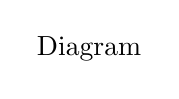
\begin{tikzpicture}
\node {Diagram};
\end{tikzpicture}
\end{center}

% Question 19
\item A particle is moving in \( x \)-\( y \) plane. At time \( t = 0 \), particle is at \( (1m, 2m) \) and has velocity \( (4 \hat{i} + 6 \hat{j}) \) m/s. At \( t = 4 \) s, particle reaches at \( (6m, 4m) \) and has velocity \( (2 \hat{i} + 10 \hat{j}) \) m/s. In the given time interval, find
\begin{enumerate}
    \item average velocity,
    \item average acceleration, and
    \item from the given data, can you find average speed?
\end{enumerate}

% Question 20
\item A stone is dropped from the top of a tower. When it crosses a point \( 5 \) m below the top, another stone is let fall from a point \( 25 \) m below the top. Both stones reach the bottom of the tower simultaneously. Find the height of the tower. Take \( g = 10 \) m/s\(^2\).

% Question 21
\item A point mass starts moving in a straight line with constant acceleration. After time \( t_0 \) the acceleration changes its sign, remaining the same in magnitude. Determine the time \( T \) from the beginning of motion in which the point mass returns to the initial position.

% Question 22
\item A football is kicked vertically upward from the ground and a student gazing out of the window sees it moving upwards past her at \( 5.00 \) m/s. The window is \( 15.0 \) m above the ground. Air resistance may be ignored. Take \( g = 10 \) m/s\(^2\).
\begin{enumerate}
    \item How high does the football go above ground?
    \item How much time does it take to go from the ground to its highest point?
\end{enumerate}

% Question 23
\item A car moving with constant acceleration covered the distance between two points \( 60.0 \) m apart in \( 6.00 \) s. Its speed as it passes the second point was \( 15.0 \) m/s.
\begin{enumerate}
    \item What is the speed at the first point?
    \item What is the acceleration?
    \item At what prior distance from the first was the car at rest?
\end{enumerate}

% Question 24
\item A particle moves along the x-direction with constant acceleration. The displacement, measured from a convenient position, is \( 2 \) m at time \( t = 0 \) and is zero when \( t = 1.0 \) s. If the velocity of the particle is momentary zero when \( t = 6 \) s, determine the acceleration \( a \) and the velocity \( v \) when \( t = 10 \) s.

% Question 25
\item At time \( t = 0 \), a particle is at \( (2m, 4m) \). It starts moving towards positive x-axis with constant acceleration \( 2 \) m/s\(^2\) (initial velocity = 0). After \( 2 \) s, an additional acceleration of \( 4 \) m/s\(^2\) starts acting on the particle in negative y-direction also. Find after next \( 2 \) s.
\begin{enumerate}
    \item velocity and
    \item coordinates of particle.
\end{enumerate}

% Question 26
\item A particle starts from the origin at \( t = 0 \) with a velocity of \( 8.0 \hat{j} \) m/s and moves in the x-y plane with a constant acceleration of \( (4.0 \hat{i} + 2.0 \hat{j}) \) m/s\(^2\). At the instant the particle’s x-coordinate is \( 29 \) m, what are
\begin{enumerate}
    \item its y-coordinate and
    \item its speed ?
\end{enumerate}

% Question 27
\item The velocity of a particle moving in a straight line is decreasing at the rate of \( 3 \) m/s per metre of displacement at an instant when the velocity is \( 10 \) m/s. Determine the time after this instant the particle at this instant.

% Question 28
\item A particle moves along a horizontal path, such that its velocity is given by \( v = (3t^2 - 6t) \) m/s, where \( t \) is the time in seconds. If it is initially located at the origin \( O \), determine the distance travelled by the particle in time interval from \( t = 0 \) to \( t = 3.5 \) s and the particle’s average velocity and average speed during the same time interval.

% Question 29
\item A particle travels in a straight line, such that for a short time \( t = 2 \) s to \( t = 6 \) s, its motion is described by \( v = (4 - 7 ln t) \) m/s, where \( v \) is in m/s\(^2\). If \( u = 6 \) m/s when \( t = 2 \) s, determine the particle’s acceleration when \( t = 3 \) s.

% Question 30
\item If the velocity \( v \) of a particle moving along a straight line decreases linearly with its displacement from \( 20 \) m/s to a value approaching zero at \( s = 30 \) m, determine the acceleration of the particle when \( s = 15 \) m.

% Question 31
\item Velocity-time graph of a particle moving in a straight line is shown in figure. At time \( t = 0 \), \( s = - 10 \) m. Plot corresponding \( a \)-\( t \) and \( s \)-\( t \) graphs.

% TikZ environment for diagram in Question 31
\begin{center}
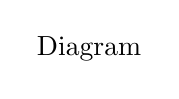
\begin{tikzpicture}
\node {Diagram};
\end{tikzpicture}
\end{center}

% Question 32
\item Velocity-time graph of a particle moving in a straight line is shown in figure. At time \( t = 0 \), \( s = 20 \) m. Plot \( a \)-\( t \) and \( s \)-\( t \) graphs of the particle.

% TikZ environment for diagram in Question 32
\begin{center}
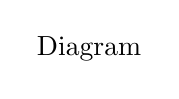
\begin{tikzpicture}
\node {Diagram};
\end{tikzpicture}
\end{center}


    \item A particle of mass \( m \) is released from a certain height \( h \) with zero initial velocity. It strikes the ground elastically (direction of its velocity is reversed but magnitude remains the same). Plot the graph between its kinetic energy and time till it returns to its initial position.
    \item A ball is dropped from a height of 80 m on a floor. At each collision, the ball loses half of its speed. Plot the speed-time graph and velocity-time graph of its motion till two collisions with the floor. \([ \text{Take} g = 10 \, \text{m/s}^2 ]\)
    \item Figure shows the acceleration-time graph of a particle moving along a straight line. After what time the particle acquires its initial velocity?

    \begin{center}
    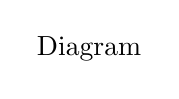
\begin{tikzpicture}
    \node {Diagram};
    \end{tikzpicture}
    \end{center}
    
    \item Velocity-time graph of a particle moving in a straight line is shown in figure. At time \( t = 0 \), displacement of the particle from mean position is 10 m. Find

    \begin{center}
    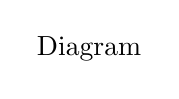
\begin{tikzpicture}
    \node {Diagram};
    \end{tikzpicture}
    \end{center}
    
    \begin{enumerate}
        \item acceleration of particle at \( t = 1 \) s, 3 s and 9 s.
        \item position of particle from mean position at \( t = 10 \) s.
        \item write down \( s-t \) equation for time interval
        \begin{enumerate}
            \item \( 0 s \leq t \leq 2 s \),
            \item \( 4 s \leq t \leq 8 s \)
        \end{enumerate}
    \end{enumerate}
    
    \item Two particles 1 and 2 are thrown in the directions shown in figure simultaneously with velocities 5 m/s and 20 m/s. Initially, particle 1 is at height 20 m from the ground. Taking upwards as the positive direction, find

    \begin{center}
    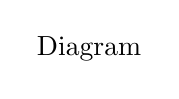
\begin{tikzpicture}
    \node {Diagram};
    \end{tikzpicture}
    \end{center}
    
    \begin{enumerate}
        \item acceleration of 1 with respect to 2
        \item initial velocity of 2 with respect to 1
        \item velocity of 1 with respect to 2 after time \( t = \frac{1}{2} \) s
        \item time when the particles will collide.
    \end{enumerate}
    
    \item A ball is thrown vertically upward from the 12 m level with an initial velocity of 18 m/s. At the same instant an open platform elevator passes the 5 m level, moving upward with a constant velocity of 2 m/s. Determine (\( g = 9.8 \, \text{m/s}^2 \))
    \begin{enumerate}
        \item when and where the ball will meet the elevator,
        \item the relative velocity of the ball with respect to the elevator when the ball hits the elevator.
    \end{enumerate}
    
    \item An automobile and a truck start from rest at the same instant, with the automobile initially at some distance behind the truck. The truck has a constant acceleration of \( 2.2 \, \text{m/s}^2 \) and the automobile has an acceleration of \( 3.5 \, \text{m/s}^2 \). The automobile overtakes the truck when it (truck) has moved 60 m.
    \begin{enumerate}
        \item How much time does it take the automobile to overtake the truck?
        \item How far was the automobile behind the truck initially?
        \item What is the speed of each during overtaking?
    \end{enumerate}

    \item Given \( |\vec{v}_{br}| = 4 \, \text{m/s} \) = magnitude of velocity of boatman with respect to river, \( v_r = 2 \, \text{m/s} \) in the direction shown. Boatman wants to reach from point A to point B. At what angle \(\theta\) should he row his boat?

    \begin{center}
    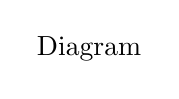
\begin{tikzpicture}
    \node {Diagram};
    \end{tikzpicture}
    \end{center}
    
    \item An aeroplane has to go from a point \( P \) to another point \( Q \), 1000 km away due north. Wind is blowing due east at a speed of 200 km/h. The air speed of plane is 500 km/h.
    \begin{enumerate}
        \item Find the direction in which the pilot should head the plane to reach the point \( Q \).
        \item Find the time taken by the plane to go from \( P \) to \( Q \).
    \end{enumerate}

    \item A train stopping at two stations 4 km apart takes 4 min on the journey from one of the station to the other. Assuming that it first accelerates with a uniform acceleration \( x \) and then that of uniform retardation \( y \), prove that \( \frac{1}{x} + \frac{1}{y} = 2 \).
\end{enumerate}






\pagebreak

\begin{center}
    \textsc{\large\textbf{Level-II}}\\
    \textsc{Single Correct Option}
\end{center}
\begin{enumerate}
    \item When a man moves down the inclined plane with a constant speed \(5 \text{ ms}^{-1}\) which makes an angle of \(37^\circ\) with the horizontal, he finds that the rain is falling vertically downward. When he moves up the same inclined plane with the same speed, he finds that the rain makes an angle \(\theta = \tan^{-1}\left(\frac{7}{8}\right)\) with the horizontal. The speed of the rain is
    \begin{tasks}(2)
        \task \(\sqrt{116} \text{ ms}^{-1}\)
        \task \(\sqrt{32}  \text{ ms}^{-1}\)
        \task \(5 \text{ ms}^{-1}\)
        \task \(\sqrt{73}  \text{ ms}^{-1}\)
    \end{tasks}

    \item Equation of motion of a body is $\frac{dv}{dt} = -4u + 8$, where \( u \) is the velocity in \( \text{ms}^{-1} \) and \( t \) is the time in second. Initial velocity of the particle was zero. Then,
    \begin{tasks}(1)
        \task the initial rate of change of acceleration of the particle is 8 \( \text{ms}^{-2} \)
        \task the terminal speed is 2 \( \text{ms}^{-1} \)
        \task Both (a) and (b) are correct
        \task Both (a) and (b) are wrong
    \end{tasks}

    \item Two particles \( A \) and \( B \) are placed in gravity free space at \( (0, 0, 0) \) m and \( (30, 0, 0) \) m respectively. Particle \( A \) is projected with a velocity \( (5\hat{i} + 10\hat{j} + 5\hat{k}) \) \( \text{ms}^{-1} \), while particle \( B \) is projected with a velocity \( (10\hat{i} + 5\hat{j} + 5\hat{k}) \) \( \text{ms}^{-1} \) simultaneously. Then,
    \begin{tasks}(2)
        \task they will collide at \( (10, 20, 10) \) m
        \task they will collide at \( (10, 10, 10) \) m
        \task they will never collide
        \task they will collide at 2 s
    \end{tasks}

    \item Velocity of the river with respect to ground is given by \( v_0 \). Width of the river is \( d \). A swimmer swims (with respect to water) perpendicular to the current with acceleration \( a = 2t \) (where \( t \) is time) starting from rest from the origin \( O \) at \( t = 0 \). The equation of trajectory of the path followed by the swimmer is
    \begin{tasks}(2)
        \task \( y = \frac{x^3}{3v_0^2} \)
        \task \( y = \frac{x^2}{2v_0^2} \)
        \task \( y = \frac{x}{v_0} \)
        \task \( y = \frac{v_0}{x} \)
    \end{tasks}

    \item The relation between time \( t \) and displacement \( x \) is \( x = ct^2 + \beta t^3 \), where \( c \) and \( \beta \) are constants. The retardation is
    \begin{tasks}(2)
        \task \( 2 ct^3 \)
        \task \( 2 \beta u^3 \)
        \task \( 2 ct\beta^3 \)
        \task \( 2 \beta^3 \)
    \end{tasks}

    \item A streetcar moves rectilinearly from station \( A \) to the next station \( B \) (from rest to rest) with an acceleration varying according to the law \( f = a - bx \), where \( a \) and \( b \) are constants and \( x \) is the distance from station \( A \). The distance between the two stations and the maximum velocity are
    \begin{tasks}(2)
        \task \( x = \frac{2a}{b}, \; v_{\text{max}} = \sqrt{\frac{a}{b}} \)
        \task \( x = \frac{b}{2a}, \; v_{\text{max}} = \sqrt{\frac{a}{b}} \)
        \task \( x = \frac{a}{2b}, \; v_{\text{max}} = \frac{b}{\sqrt{a}} \)
        \task \( x = \frac{a}{b}, \; v_{\text{max}} = \sqrt{\frac{b}{a}} \)
    \end{tasks}

    \item A particle of mass \( m \) moves on positive \( x \)-axis under the influence of force acting towards the origin given by \( -kx^2 \). If the particle starts from rest at \( x = a \), the speed it will attain when it crosses the origin is
    \begin{tasks}(2)
        \task \( \sqrt{\frac{k}{ma}} \)
        \task \( \sqrt{\frac{2k}{ma}} \)
        \task \( \sqrt{\frac{ma}{2k}} \)
        \task None of these
    \end{tasks}

    \item A particle is moving along a straight line whose velocity-displacement graph is as shown in the figure. What is the magnitude of acceleration when displacement is 3 m?
    \begin{tasks}(2)
        \task $\frac{4}{3}$ ms\textsuperscript{-2}
        \task $\frac{3\sqrt{3}}{\sqrt{3}}$ ms\textsuperscript{-2}
        \task $\frac{\sqrt{3}}{3}$ ms\textsuperscript{-2}
        \task $\frac{4}{3}$ ms\textsuperscript{-2}
    \end{tasks}

    \item A particle is falling freely under gravity. In first t second it covers distance $x_1$, and in the next t second, it covers distance $x_2$, then t is given by
    \begin{tasks}(2)
        \task $\frac{x_2 - x_1}{g}$
        \task $\frac{x_1 + x_2}{g}$
        \task $\sqrt{\frac{2(x_2 - x_1)}{g}}$
        \task $\frac{1}{2}(x_2 + x_1)$
    \end{tasks}

    \item A rod AB is shown in figure. End A of the rod is fixed on the ground. Block is moving with velocity 2 ms\textsuperscript{-1} towards right. The velocity of end B of rod at the instant shown in figure is
    \begin{tasks}(2)
        \task $\frac{3}{\sqrt{3}}$ ms\textsuperscript{-1}
        \task 2 ms\textsuperscript{-1}
        \task $\frac{2}{3}$ ms\textsuperscript{-1}
        \task 4 ms\textsuperscript{-1}
    \end{tasks}
    
    \item A motorcycle in a stolen car passes through a police check post at his top speed of 90 kmh\textsuperscript{-1}. A motorcycl\textsuperscript{1} cop, reacting after 2 s, accelerates from rest at 5 ms\textsuperscript{-2}. His top speed being 108 kmh\textsuperscript{-1}. Find the maximum separation between policemen and thief.
    \begin{tasks}(2)
        \task 115 m
        \task 110.56 m
        \task 116 m
        \task None of these
    \end{tasks}
    
    \item Anoop (A) hits a ball along the ground with a speed u in a direction which makes an angle 30\textdegree{} with the line joining him and the fiedler Baul (B). Baul runs to intercept the ball with a speed $2u/3$. At what angle $\theta$ should he run to intercept the ball?
    \begin{tasks}(4)
        \task $\sin^{-1}\left[\frac{\sqrt{3}}{2}\right]$
        \task $\sin^{-1}\left[\frac{2}{3}\right]$
        \task $\sin^{-1}\left[\frac{1}{3}\right]$
        \task $\sin^{-1}\left[\frac{1}{4}\right]$
    \end{tasks}

    \item A car is travelling on a straight road. The maximum velocity the car can attain is 24 ms\textsuperscript{-1}. The maximum acceleration and deceleration it can attain are 1 ms\textsuperscript{-2} and 4 ms\textsuperscript{-2} respectively. The shortest time the car takes from rest to rest in a distance of 200 m is,
    \begin{tasks}(2)
        \task 22.4 s
        \task 30 s
        \task 11.2 s
        \task 5.6 s
    \end{tasks}
    
    \item A car is travelling on a road. The maximum velocity the car can attain is 24 ms\textsuperscript{-1} and the maximum deceleration is 4 ms\textsuperscript{-2}. If car starts from rest and comes to rest after travelling 1032 m in the shortest time of 56 s, the maximum acceleration that the car can attain is
    \begin{tasks}(2)
        \task 6 ms\textsuperscript{-2}
        \task 1.2 ms\textsuperscript{-2}
        \task 12 ms\textsuperscript{-2}
        \task 3.6 ms\textsuperscript{-2}
    \end{tasks}

    \item Two particles are moving along two straight lines in and the same plane with same speed equal to 20 cm/s. The angle between the two lines is 60\textdegree{}, their intersection point is O. At a certain moment, the two particles are located at distances 3m and 4m from O and are moving towards O. Subsequently, the shortest distance between them will be
    \begin{tasks}(2)
        \task 50 cm
        \task $40\sqrt{2}$ cm
        \task $50\sqrt{2}$ cm
        \task $50\sqrt{3}$ cm
    \end{tasks}
\end{enumerate}

\begin{center}
    \textsc{More than one correct option may be correct.}
\end{center}
\begin{enumerate}
    \item A particle having a velocity \( v = u_0 \) at \( t = 0 \) is decelerated at the rate \( |a| = \alpha \sqrt{v} \), where \( \alpha \) is a positive constant.
    \begin{tasks}(1)
        \task The particle comes to rest at \( t = \frac{2}{\alpha} \sqrt{u_0} \)
        \task The particle will come to rest at infinity
        \task The distance travelled by the particle before coming to rest is \( \frac{2u_0^{3/2}}{\alpha} \)
        \task The distance travelled by the particle before coming to rest is \( \frac{2u_0^{3/2}}{3\alpha} \)
    \end{tasks}

    \item At time \( t = 0 \), a car moving along a straight line has a velocity of 16 m/s\(^{-1}\). It slows down with an acceleration of \( -0.5 \) m/s\(^2\), where \( t \) is in second. Mark the correct statement(s).
    \begin{tasks}(1)
        \task The direction of velocity changes at \( t = 8 \) s
        \task The distance travelled in 4 s is approximately 58.67 m
        \task The distance travelled by the particle in 10 s is 94 m
        \task The speed of particle at \( t = 10 \) s is 9 m/s\(^{-1}\)
    \end{tasks}

    \item An object moves with constant acceleration \( a \). Which of the following expressions are also constant?
    \begin{tasks}(2)
        \task \( a \)
        \task \( \frac{dv}{dt} \)
        \task \( \frac{d(v^2)}{dt} \)
        \task \( \frac{d}{dt} \left( \frac{v}{|v|} \right) \)
    \end{tasks}

    \item Ship A is located 4 km north and 3 km east of ship B. Ship A has a velocity of 20 kmh\(^{-1}\) towards the south and ship B is moving at 40 kmh\(^{-1}\) in a direction 37\(^{\circ}\) north of east. X and Y-axes are along east and north directions, respectively
    \begin{tasks}(1)
        \task Velocity of A relative to B is \( -32i - 44j \) km/h
        \task Position of A relative to B as a function of time is given by \( r_{AB} = (3t - 32)i + (4 - 44j)t \) km
        \task Velocity of A relative to B is \( 32i - 44j \) km/h
        \task Position of A relative to B as a function of time is given by \( (32i + (4 - 44j)t \) km
    \end{tasks}

    \item Starting from rest a particle is first accelerated for time \( t_1 \) with constant acceleration \( a_1 \) and then stops in time \( t_2 \) with constant retardation \( a_2 \). Let \( u_1 \) be the average velocity in this case and \( s_1 \) the total displacement. In the second case it is accelerating for the same time \( t_1 \) with constant acceleration \( 2a_1 \) and come to rest with constant retardation \( a_2 \) in time \( t_3 \). If \( u_2 \) is the average velocity in this case and \( s_2 \) the total displacement, then
    \begin{tasks}(2)
        \task \( u_2 = 2u_1 \)
        \task \( u_1 < u_2 < 4u_1 \)
        \task \( s_2 = 2s_1 \)
        \task \( 2s_1 < s_2 < 4s_1 \)
    \end{tasks}

    \item A particle is moving along a straight line. The displacement of the particle becomes zero in a certain time \( t > 0 \). The particle does not undergo any collision.
    \begin{tasks}(1)
        \task The acceleration of the particle may be zero always
        \task The acceleration of the particle may be uniform
        \task The velocity of the particle must be zero at some instant
        \task The acceleration of the particle must change its direction
    \end{tasks}

    \item A particle is resting over a smooth horizontal floor. At \(t = 0\), a horizontal force starts acting on it. Magnitude of the force increases with time according to law \(F = \alpha t\), where \(\alpha\) is a positive constant. From figure, which of the following statements are correct?
    \begin{tasks}(1)
      \task Curve 1 can be the plot of acceleration against time
      \task Curve 2 can be the plot of velocity against time
      \task Curve 2 can be the plot of velocity against acceleration
      \task Curve 1 can be the plot of displacement against time
    \end{tasks}
    
    \item A train starts from rest at \(S = 0\) and is subjected to an acceleration as shown in figure. Then,
    \begin{tasks}(1)
      \task velocity at the end of 10 m displacement is 20 m\(^{-1}\)
      \task velocity of the train at \(S = 10\) m is 10 m\(^{-1}\)
      \task The maximum velocity attained by train is \(\sqrt{180}\) m\(^{-1}\)
      \task The maximum velocity attained by the train is 15 m\(^{-1}\)
    \end{tasks}
    
    \item For a moving particle, which of the following options may be correct?
    \begin{tasks}(2)
      \task \(|V_{av}| < v_{av}\)
      \task \(|V_{av}| > v_{av}\)
      \task \(V_{av} = 0\) but \(v_{av} \neq 0\)
      \task \(v_{av} = 0\) but \(V_{av} \neq 0\)
    \end{tasks}
    
    \item Identify the correct graph representing the motion of a particle along a straight line with constant acceleration with zero initial velocity.
    % Insert TikZ code or image here, represented by figures (a), (b), (c), and (d)
    
    \item A man who can swim at a velocity \(v\) relative to water wants to cross a river of width \(b\), flowing with a speed \(u\).
    \begin{tasks}(1)
      \task The minimum time in which he can cross the river is \(\frac{b}{v}\)
      \task He can reach a point exactly opposite on the bank in time \(t = \frac{b}{\sqrt{v^2 - u^2}}\) if \(v > u\)
      \task He cannot reach the point exactly opposite on the bank if \(u > v\)
      \task He cannot reach the point exactly opposite on the bank if \(u \geq v\)
    \end{tasks}
  
    \item The figure shows the velocity \((v)\) of a particle plotted against time \((t)\). 
    \begin{tikzpicture}[scale=0.8]
        \draw[->] (0,0) -- (4,0) node[anchor=north] {$t$};
        \draw[->] (0,0) -- (0,3) node[anchor=east] {$v$};
        \draw (0,0) -- (1.5,2) -- (3,0);
        \draw[dashed] (1.5,2) -- (1.5,0) node[anchor=north] {$T$};
        \draw[dashed] (3,0) -- (3,2) node[anchor=west] {$2T$};
    \end{tikzpicture}
    \begin{tasks}(1)
        \task The particle changes its direction of motion at some point
        \task The acceleration of the particle remains constant
        \task The displacement of the particle is zero
        \task The initial and final speeds of the particle are the same
    \end{tasks}
    
    \item The speed of a train increases at a constant rate \(\alpha\) from zero to \(u\) and then remains constant for an interval and finally decreases to zero at a constant rate \(\beta\). The total distance travelled by the train is \(l\). The time taken to complete the journey is \(t\). Then,
    \begin{tasks}(2)
        \task \( t = \dfrac{l}{u} + \dfrac{\alpha + \beta}{\alpha \beta} \)
        \task \( t = \dfrac{l}{u} + u \left( \dfrac{1}{2 \alpha} + \dfrac{1}{2 \beta} \right) \)
        \task \( t \) is minimum when \( u = \dfrac{2l}{\alpha \beta} \sqrt{\dfrac{\alpha}{\alpha + \beta}} \)
        \task \( t \) is minimum when \( u = \dfrac{2l}{\alpha \beta} \sqrt{\dfrac{\alpha + \beta}{\alpha}} \)
    \end{tasks}
    
    \item A particle moves in \(x\)-\(y\) plane and at time \(t\) is at the point \((t^2, t^3 - 2t)\), then which of the following is/are correct?
    \begin{tasks}(1)
        \task At \( t = 0 \), particle is moving parallel to \(y\)-axis
        \task At \( t = 0 \), direction of velocity and acceleration are perpendicular
        \task At \( t = \dfrac{1}{\sqrt{3}} \), particle is moving parallel to \(x\)-axis
        \task At \( t = 0 \), particle is at rest
    \end{tasks}
    
    \item A car is moving with uniform acceleration along a straight line between two stops \(X\) and \(Y\). Its speed at \(X\) and at mid-point \(XY\) is 10 m/s,
    \begin{tasks}(1)
        \task its speed at a point \(A\) such that \(XA : AY = 1 : 3\) is 5 m/s
        \task the time to go from \(X\) to the mid-point of \(XY\) is double of that to go from mid-point to \(Y\)
        \task the distance travelled in first half of the total time is half of the distance travelled in the second half of the time
        \task the speed at \(Y\) are 2 m/s and 14 m/s, Then
    \end{tasks}
    \end{enumerate}


\pagebreak


\begin{center}
    \textsc{Comprehension-I}
\end{center}
An elevator without a ceiling is ascending up with an acceleration of $5 \, \text{ms}^{-2}$. A boy on the elevator shoots a ball in vertical upward direction from a height of $2\, \text{m}$ above the floor of the elevator. At this instant the elevator is moving up with a velocity of $10\, \text{ms}^{-1}$ and floor of the elevator is at a height of $50\, \text{m}$ from the ground. The initial speed of the ball is $15\, \text{ms}^{-1}$ with respect to the elevator. Consider the duration for which the ball strikes the floor of the elevator in answering the following questions. ($g = 10 \, \text{ms}^{-2}$)

\begin{enumerate}
    \item The time in which the ball strikes the floor of the elevator is given by
    	\begin{tasks}(4)
    		\task $2.13 \, \text{s}$
    		\task $2.0 \, \text{s}$
    		\task $1.0 \, \text{s}$
    		\task $3.12 \, \text{s}$
    	\end{tasks}
    	
    \item The maximum height reached by ball, as measured from the ground would be
    	\begin{tasks}(4)
    		\task $73.65 \, \text{m}$
    		\task $116.25 \, \text{m}$
    		\task $82.56 \, \text{m}$
    		\task $63.25 \, \text{m}$
    	\end{tasks}
    	
    \item Displacement of ball with respect to ground during its flight would be
    	\begin{tasks}(4)
    		\task $16.25 \, \text{m}$
    		\task $8.76 \, \text{m}$
    		\task $20.24 \, \text{m}$
    		\task $30.56 \, \text{m}$
    	\end{tasks}
    	
    \item The maximum separation between the floor of elevator and the ball during its flight would be
    	\begin{tasks}(4)
    		\task $12 \, \text{m}$
    		\task $15 \, \text{m}$
    		\task $9.5 \, \text{m}$
    		\task $7.5 \, \text{m}$
    	\end{tasks}
\end{enumerate}

\vspace*{10 mm}

\begin{center}
    \textsc{Comprehension-II}
\end{center}
A situation is shown in which two objects A and B start their motion from same point in same direction. The graph of their velocities against time is drawn. $u_A$ and $u_B$ are the initial velocities of A and B respectively. T is the time at which their velocities become equal after start of motion. You cannot use the data of one question while solving another question of the same set. So all the questions are independent of each other.

\begin{enumerate}
    \item If the value of T is 4 s, then the time after which A will meet B is
        \begin{tasks}(4)
            \task 12 s
            \task 6 s
            \task 8 s
            \task data insufficient
        \end{tasks}

    \item Let $u_A$ and $u_B$ be the velocities of the particles A and B respectively at the moment A and B meet after start of the motion. If $u_A = 5 \text{ ms}^{-1}$ and $u_B = 15 \text{ ms}^{-1}$, then the magnitude of the difference of velocities $u_A$ and $u_B$ is
        \begin{tasks}(4)
            \task 5 ms\(^{-1}\)
            \task 15 ms\(^{-1}\)
            \task 10 ms\(^{-1}\)
            \task data insufficient
        \end{tasks}

    \item After 10 s of the start of motion of both objects A and B, find the value of velocity of A if $u_A = 6 \text{ ms}^{-1}$, $u_B = 12 \text{ ms}^{-1}$ and at T velocity of A is 8 ms\(^{-1}\) and T = 4 s
        \begin{tasks}(4)
            \task 12 ms\(^{-1}\)
            \task 10 ms\(^{-1}\)
            \task 15 ms\(^{-1}\)
            \task None of these
        \end{tasks}
\end{enumerate}

\vspace*{10 mm}


\begin{enumerate}
    \item Match the following two columns:
    \begin{center}
        \renewcommand{\arraystretch}{2}
        \begin{table}[h]
            \centering
            \begin{tabular}{p{0.25cm}p{7cm}|p{0.25cm}p{6cm}}
            \hline
            & Column I & &Column II \\
            \hline
            (a)& 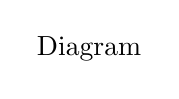
\begin{tikzpicture}[scale=0.5]
                    \node {Diagram};
                 \end{tikzpicture} & (p) &speed must be increasing \\
            (b)& 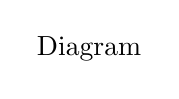
\begin{tikzpicture}[scale=0.5]
                    \node {Diagram};
                 \end{tikzpicture} & (q) &speed must be decreasing \\
            (c)& 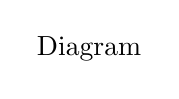
\begin{tikzpicture}[scale=0.5]
                    \node {Diagram};
                 \end{tikzpicture} & (r) &speed may be increasing \\
            (d)& 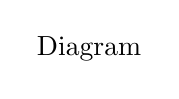
\begin{tikzpicture}[scale=0.5]
                    \node {Diagram};
                 \end{tikzpicture} & (s) &speed may be decreasing \\
            \hline
            \end{tabular}
        \end{table}
    \end{center}

    \pagebreak
    
    \item Match the following two columns:
    \begin{center}
        \renewcommand{\arraystretch}{2}
        \begin{table}[h]
            \centering
            \begin{tabular}{p{0.25cm}p{7cm}|p{0.25cm}p{6cm}}
            \hline
            & Column I & &Column II \\
            \hline
            (a)& \( \vec{v} = -2\hat{i}, \vec{a} = -4\hat{j} \) & (p) &speed increasing \\
            (b)& \( \vec{v} = 2\hat{i}, \vec{a} = 2\hat{i} + 2\hat{j} \) & (q) &speed decreasing \\
            (c)& \( \vec{v} = -2\hat{i}, \vec{a} = +2\hat{i} \) & (r) &speed constant \\
            (d)& \( \vec{v} = 2\hat{i}, \vec{a} = -2\hat{i} + 2\hat{j} \) & (s) &Nothing can be said \\
            \hline
            \end{tabular}
        \end{table}
    \end{center}
    
    \item The velocity-time graph of a particle moving along X-axis is shown in figure. Match the entries of Column I with the entries of Column II. 
    
    \begin{center}
        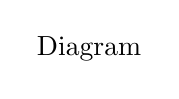
\begin{tikzpicture}
            \node {Diagram};
        \end{tikzpicture}
    \end{center}

    \begin{center}
        \renewcommand{\arraystretch}{2}
        \begin{table}[h]
            \centering
            \begin{tabular}{p{0.25cm}p{5cm}|p{0.25cm}p{8cm}}
            \hline
            & Column I & & Column II \\
            \hline
            (a) & For AB, particle is & (p) & Moving in +ve X-direction with increasing speed \\
            (b) & For BC, particle is & (q) & Moving in +ve X-direction with decreasing speed \\
            (c) & For CD, particle is & (r) & Moving in -ve X-direction with increasing speed \\
            (d) & For DE, particle is & (s) & Moving in -ve X-direction with decreasing speed \\
            \hline
            \end{tabular}
        \end{table}
    \end{center}
    
    \item Corresponding to velocity-time graph in one dimensional motion of a particle as shown in figure, match the following two columns.
    
    \begin{center}
        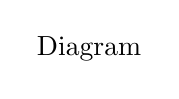
\begin{tikzpicture}
            \node {Diagram};
        \end{tikzpicture}
    \end{center}
    
    \begin{center}
        \renewcommand{\arraystretch}{2}
        \begin{table}[h]
            \centering
            \begin{tabular}{p{0.25cm}p{7cm}|p{0.25cm}p{6cm}}
            \hline
            & Column I & & Column II \\
            \hline
            (a) & Average velocity between zero second and 4 s & (p) & 10 SI units \\
            (b) & Average acceleration between 1 s and 4 s & (q) & 2.5 SI units \\
            (c) & Average speed between zero second and 6 s & (r) & 5 SI units \\
            (d) & Rate of change of speed at 4 s & (s) & None of the above \\
            \hline
            \end{tabular}
        \end{table}
    \end{center}

    \pagebreak
    
    \item A particle is moving along x-axis. Its x-coordinate varies with time as: $x = -20 + 5t^2$.
    
    For the given equation match the following two columns:
    
    \begin{center}
        \renewcommand{\arraystretch}{2}
        \begin{table}[h]
            \centering
            \begin{tabular}{p{0.25cm}p{8cm}|p{0.25cm}p{5cm}}
            \hline
            & Column I & & Column II \\
            \hline
            (a) & Particle will cross the origin at & (p) & zero second \\
            (b) & At what time velocity and acceleration are equal & (q) & 1 s \\
            (c) & At what time particle changes its direction of motion & (r) & 2 s \\
            (d) & At what time velocity is zero & (s) & None of the above \\
            \hline
            \end{tabular}
        \end{table}
    \end{center}

    \item x and y-coordinates of a particle moving in x-y plane are, \( x = 1 - 2t + t^2 \) and \( y = 4 - 4t + t^2 \)

  For the given situation match the following two columns:
  
  \begin{center}
      \renewcommand{\arraystretch}{2}
      \begin{table}[h]
          \centering
          \begin{tabular}{p{0.25cm}p{8cm}|p{0.25cm}p{5cm}}
          \hline
          & Column I & &Column II \\
          \hline
          (a)& y-component of velocity when it crosses the y-axis & (p) & \( + 2 \) SI units \\
          (b)& x-component of velocity when it crosses the x-axis & (q) & \( - 2 \) SI units \\
          (c)& Initial velocity of particle & (r) & \( + 4 \) SI units \\
          (d)& Initial acceleration of particle & (s) & None of the above \\
          \hline
          \end{tabular}
      \end{table}
  \end{center}
\end{enumerate}
  

\begin{center}
    \textsc{Subjective Questions}
\end{center}

\begin{enumerate}
    \item To test the quality of a tennis ball, you drop it onto the floor from a height of 4.00 m. It rebounds to a height of 2.00 m. If the ball is in contact with the floor for 12.0 ms, what is its average acceleration during that contact? Take \( g = 9.8 \text{ m/s}^2 \).
    
    \item The acceleration-displacement graph of a particle moving in a straight line is as shown in figure, initial velocity of particle is zero. Find the velocity of the particle when displacement of the particle is \( s = 12 \text{ m} \).
    \begin{center}
        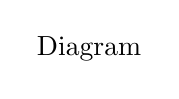
\begin{tikzpicture}
            \node {Diagram};
        \end{tikzpicture}
    \end{center}
    
    \item At the initial moment three points \( A, B \) and \( C \) are on a horizontal straight line at equal distances from one another. Point \( A \) begins to move vertically upward with a constant velocity \( v \) and point \( C \) vertically downward without any initial velocity but with a constant acceleration \( a \). How should point \(
B \) move vertically for all the three points to be constantly on one straight line. The points begin to move simultaneously.
    
    \item A particle moves in a straight line with constant acceleration \( a \). The displacements of particle from origin in times \( t_1, t_2 \) and \( t_3 \) are \( s_1, s_2 \) and \( s_3 \) respectively. If times are in AP with common difference \( d \) and displacements are in GP, then prove that \( a = \frac{\left( \sqrt{s_1} - \sqrt{s_3}
\right)^2}{d^2} \).
    
    \item A car is to be hoisted by elevator to the fourth floor of a parking garage, which is 14 m above the ground. If the elevator can have maximum acceleration of 0.2 m/s\(^2\) and maximum deceleration of 0.1 m/s\(^2\) and can reach a maximum speed of 2.5 m/s, determine the shortest time to make the lift, starting from rest and ending at 
rest.
    
    \item To stop a car, first you require a certain reaction time to begin braking; then the car slows under the constant braking deceleration. Suppose that the total distance moved by your car during these two phases is 56.7 m when its initial speed is 80.5 km/h and 24.4 m when its initial speed is 48.3 km/h. What are \\
    (a) your reaction time and \\
    (b) the magnitude of the deceleration?

    \item An elevator without a ceiling is ascending with a constant speed of 10 m/s. A boy on the elevator shoots a ball directly upward, from a height of 2.0 m above the elevator floor. At this time the elevator floor is 28 m above the ground. The initial speed of the ball with respect to the elevator is 20 m/s. (Take \( g = 9.8 \, m/s^2 \))
    \begin{enumerate}
        \item What maximum height above the ground does the ball reach?
        \item How long does the ball take to return to the elevator floor?
    \end{enumerate}
    \item A particle moves along a straight line and its velocity depends on time as \( v = 3t - t^2 \). Here, \( v \) is in m/s and \( t \) in second. Find
    \begin{enumerate}
        \item average velocity
        \item average speed for first five seconds.
    \end{enumerate}
    \item The acceleration of particle varies with time as shown.
    \begin{center}
        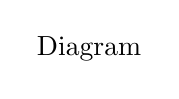
\begin{tikzpicture}
            \node {Diagram};
        \end{tikzpicture}
    \end{center}
    \begin{enumerate}
        \item Find an expression for velocity in terms of \( t \).
        \item Calculate the displacement of the particle in the time interval from \( t = 2s \) to \( t = 4s \).
    \end{enumerate}
    \item A man wishes to cross a river of width 120 m by a motorboat. His rowing speed in still water is 3 m/s and his maximum walking speed is 1 m/s. The river flows with velocity of 4 m/s.
    \begin{enumerate}
        \item Find the path which he should take to get to the point directly opposite to his starting point in the shortest time.
        \item Also, find the time which he takes to reach his destination.
    \end{enumerate}
    \item The current velocity of river grows in proportion to the distance from its bank and reaches the maximum value \( u_0 \) in the middle. Near the banks the velocity is zero. A boat is moving along the river in such a manner that the boatman rows his boat always perpendicular to the current. The speed of the boat in still water is \( u \). Find the distance through which the boat crossing the river will be carried away by the current, if the width of the river is \( c \). Also determine the trajectory of the boat.
    \item The \( v-s \) graph for an airplane travelling on a straight runway is shown. Determine the acceleration of the plane at \( s = 50 m \) and \( s = 150 m \). Draw the \( a-s \) graph.
    \begin{center}
        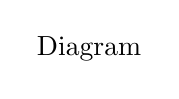
\begin{tikzpicture}
            \node {Diagram};
        \end{tikzpicture}
    \end{center}

    
    \item A river of width \( a \) with straight parallel banks flows due north with speed \( u \). The points \( O \) and \( A \) are on opposite banks and \( A \) is due east of \( O \). Coordinate axes \( O_x \) and \( O_y \) are taken in the east and north directions respectively. A boat, whose speed is \( v \) relative to water, starts from \( O \) and crosses the river. If the boat is steered due east and \( u \) varies with \( x \) as: \( u = u(x-a) \to \frac{u}{x^2} \). Find
    \begin{enumerate}
        \item equation of trajectory of the boat,
        \item time taken to cross the river,
        \item absolute velocity of boatman when he reaches the opposite bank,
        \item the displacement of boatman when he reaches the opposite bank from the initial position.
    \end{enumerate}
    
    \item A river of width \( a \) is flowing with a uniform velocity \( u \). A boat starts moving from point \( P \) also with velocity \( u \) relative to the river. The direction of resultant velocity is always perpendicular to the line joining boat and the fixed point \( R \). Point \( Q \) is on the opposite side of the river. \( P, Q \) and \( R \) are in a straight line. If \( PQ = QR = a \), find (a) the trajectory of the boat, (b) the drifting of the boat and (c) the time taken by the boat to cross the river.
    \begin{center}
        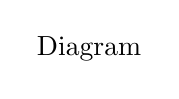
\begin{tikzpicture}
            \node {Diagram};
        \end{tikzpicture}
    \end{center}

    \item The \( u-s \) graph describing the motion of a motorcycle is shown in Figure. Construct the \( u-s \) graph of the motion and determine the time needed for the motorcycle to reach the position \( s = 120 \) m. Given \( n = 1.6 \).
    \begin{center}
        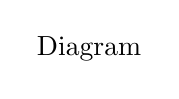
\begin{tikzpicture}
            \node {Diagram};
        \end{tikzpicture}
    \end{center}
    
    \item The jet plane starts from rest at \( s = 0 \) and is subjected to the acceleration shown. Determine the speed of the plane when it has traveled 60 m.
    \begin{center}
        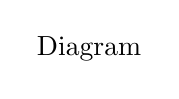
\begin{tikzpicture}
            \node {Diagram};
        \end{tikzpicture}
    \end{center}
    
    \item A particle leaves the origin with an initial velocity \( \mathbf{v} = (3.00\hat{i}) \) m/s and a constant acceleration \( \mathbf{a} = (-1.00\hat{i} - 0.500\hat{j}) \) m/s\(^2\). When the particle reaches its maximum \( x \) coordinate, what are
    \begin{enumerate}
        \item its velocity and 
        \item its position vector?
    \end{enumerate}
    
    \item The speed of a particle moving in a plane is equal to the magnitude of its instantaneous velocity,
    
    \[ u = | \mathbf{v} | = \sqrt{v_x^2 + v_y^2}. \]
    \begin{enumerate}
        \item Show that the rate of change of the speed is given by
    
        \[ \frac{du}{dt} = \frac{(v_xa_x + v_ya_y)}{\sqrt{v_x^2 + v_y^2}}. \]
    
        \item Show that the rate of change of speed can be expressed as \( \frac{du}{dt} = \mathbf{v} \cdot \mathbf{a_u} \), and use this result to explain why \( \frac{du}{dt} \) is equal to \( a_t \), the component of \( \mathbf{a} \) that is parallel to \( \mathbf{v} \).
    \end{enumerate}
    
    \item A man with some passengers in his boat, starts perpendicular to flow of river 200 m wide and flowing with 2 m/s. Speed of boat in still water is 4 m/s. When he reaches half the width of river the passengers asked him that they want to reach the just opposite end from where they have started.
    \begin{enumerate}
        \item Find the direction due which he must row to reach the required end.
        \item How many times more time, it would take to that if he would have denied the passengers?
    \end{enumerate}
    
    \item A child in danger of drowning in a river is being carried downstream by a current that flows uniformly at a speed of 2.5 km/h. The child is 0.6 km from shore and 0.8 km upstream of a boat landing when a rescue boat sets out. If the boat proceeds at its maximum speed of 20 km/h with respect to the water, what angle does the boat velocity \( \mathbf{u} \) make with the shore? How long will it take boat to reach the child?
    
    \item A launch plies between two points \( A \) and \( B \) on the opposite banks of a river always following the line \( AB \). The distance \( S \) between points \( A \) and \( B \) is 200 m. The velocity of the river current \( \mathbf{u} = 1.9 \) m/s is constant over the entire width of the river. The line \( AB \) makes an angle \( \alpha = 60^\circ \) with the direction of the current. With what velocity \( u \) and with what angle \( \beta \) to the line \( AB \) should the launch move to cover the distance \( AB \) and back in a time \( t = 5 \) min? The angle \( \beta \) remains the same during the passage from \( A \) to \( B \) and from \( B \) to \( A \).
    
    \item The slopes of wind screen of two cars are \( \alpha_1 = 30^\circ \) and \( \alpha_2 = 15^\circ \) respectively. At what ratio \( u_1/u_2 \) of the velocities of the cars will their drivers see the hail stones bounced back by the wind screen on their cars in vertical direction? Assume hail stones fall vertically downwards and collisions to be elastic.
    
    \item A projectile of mass \( m \) is fired into a liquid at an angle \( \theta_0 \) with an initial velocity \( u_0 \) as shown. If the liquid develops a frictional or drag resistance on the projectile which is proportional to its velocity, i.e. \( \mathbf{F} = -k\mathbf{v} \) where \( k \) is a positive constant, determine the \( x \) and \( y \) components of its velocity at any instant. Also find the maximum distance \( x_{\text{max}} \) that it travels.
    \begin{center}
        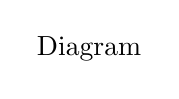
\begin{tikzpicture}
            \node {Diagram};
        \end{tikzpicture}
    \end{center}
    
    \item A man in a boat crosses a river from point \( A \). If he rows perpendicular to the banks he reaches point \( C \) ( \( BC = 120 \) m) in 10 min. If the man heads at a certain angle \( \alpha \) to the straight line \( AB \) ( \( AB \) is perpendicular to the banks) against the current he reaches point \( B \) in 12.5 min. Find the width of the river \( u \), the rowing velocity \( v \), the speed of the river current \( w \) and the angle \( \alpha \). Assume the velocity of the boat relative to water to be constant and the same magnitude in both cases.

    \begin{center}
        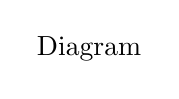
\begin{tikzpicture}
            \node {Diagram};
        \end{tikzpicture}
    \end{center}
\end{enumerate}



\end{document}